\begin{figure}[h!]
    \centering
    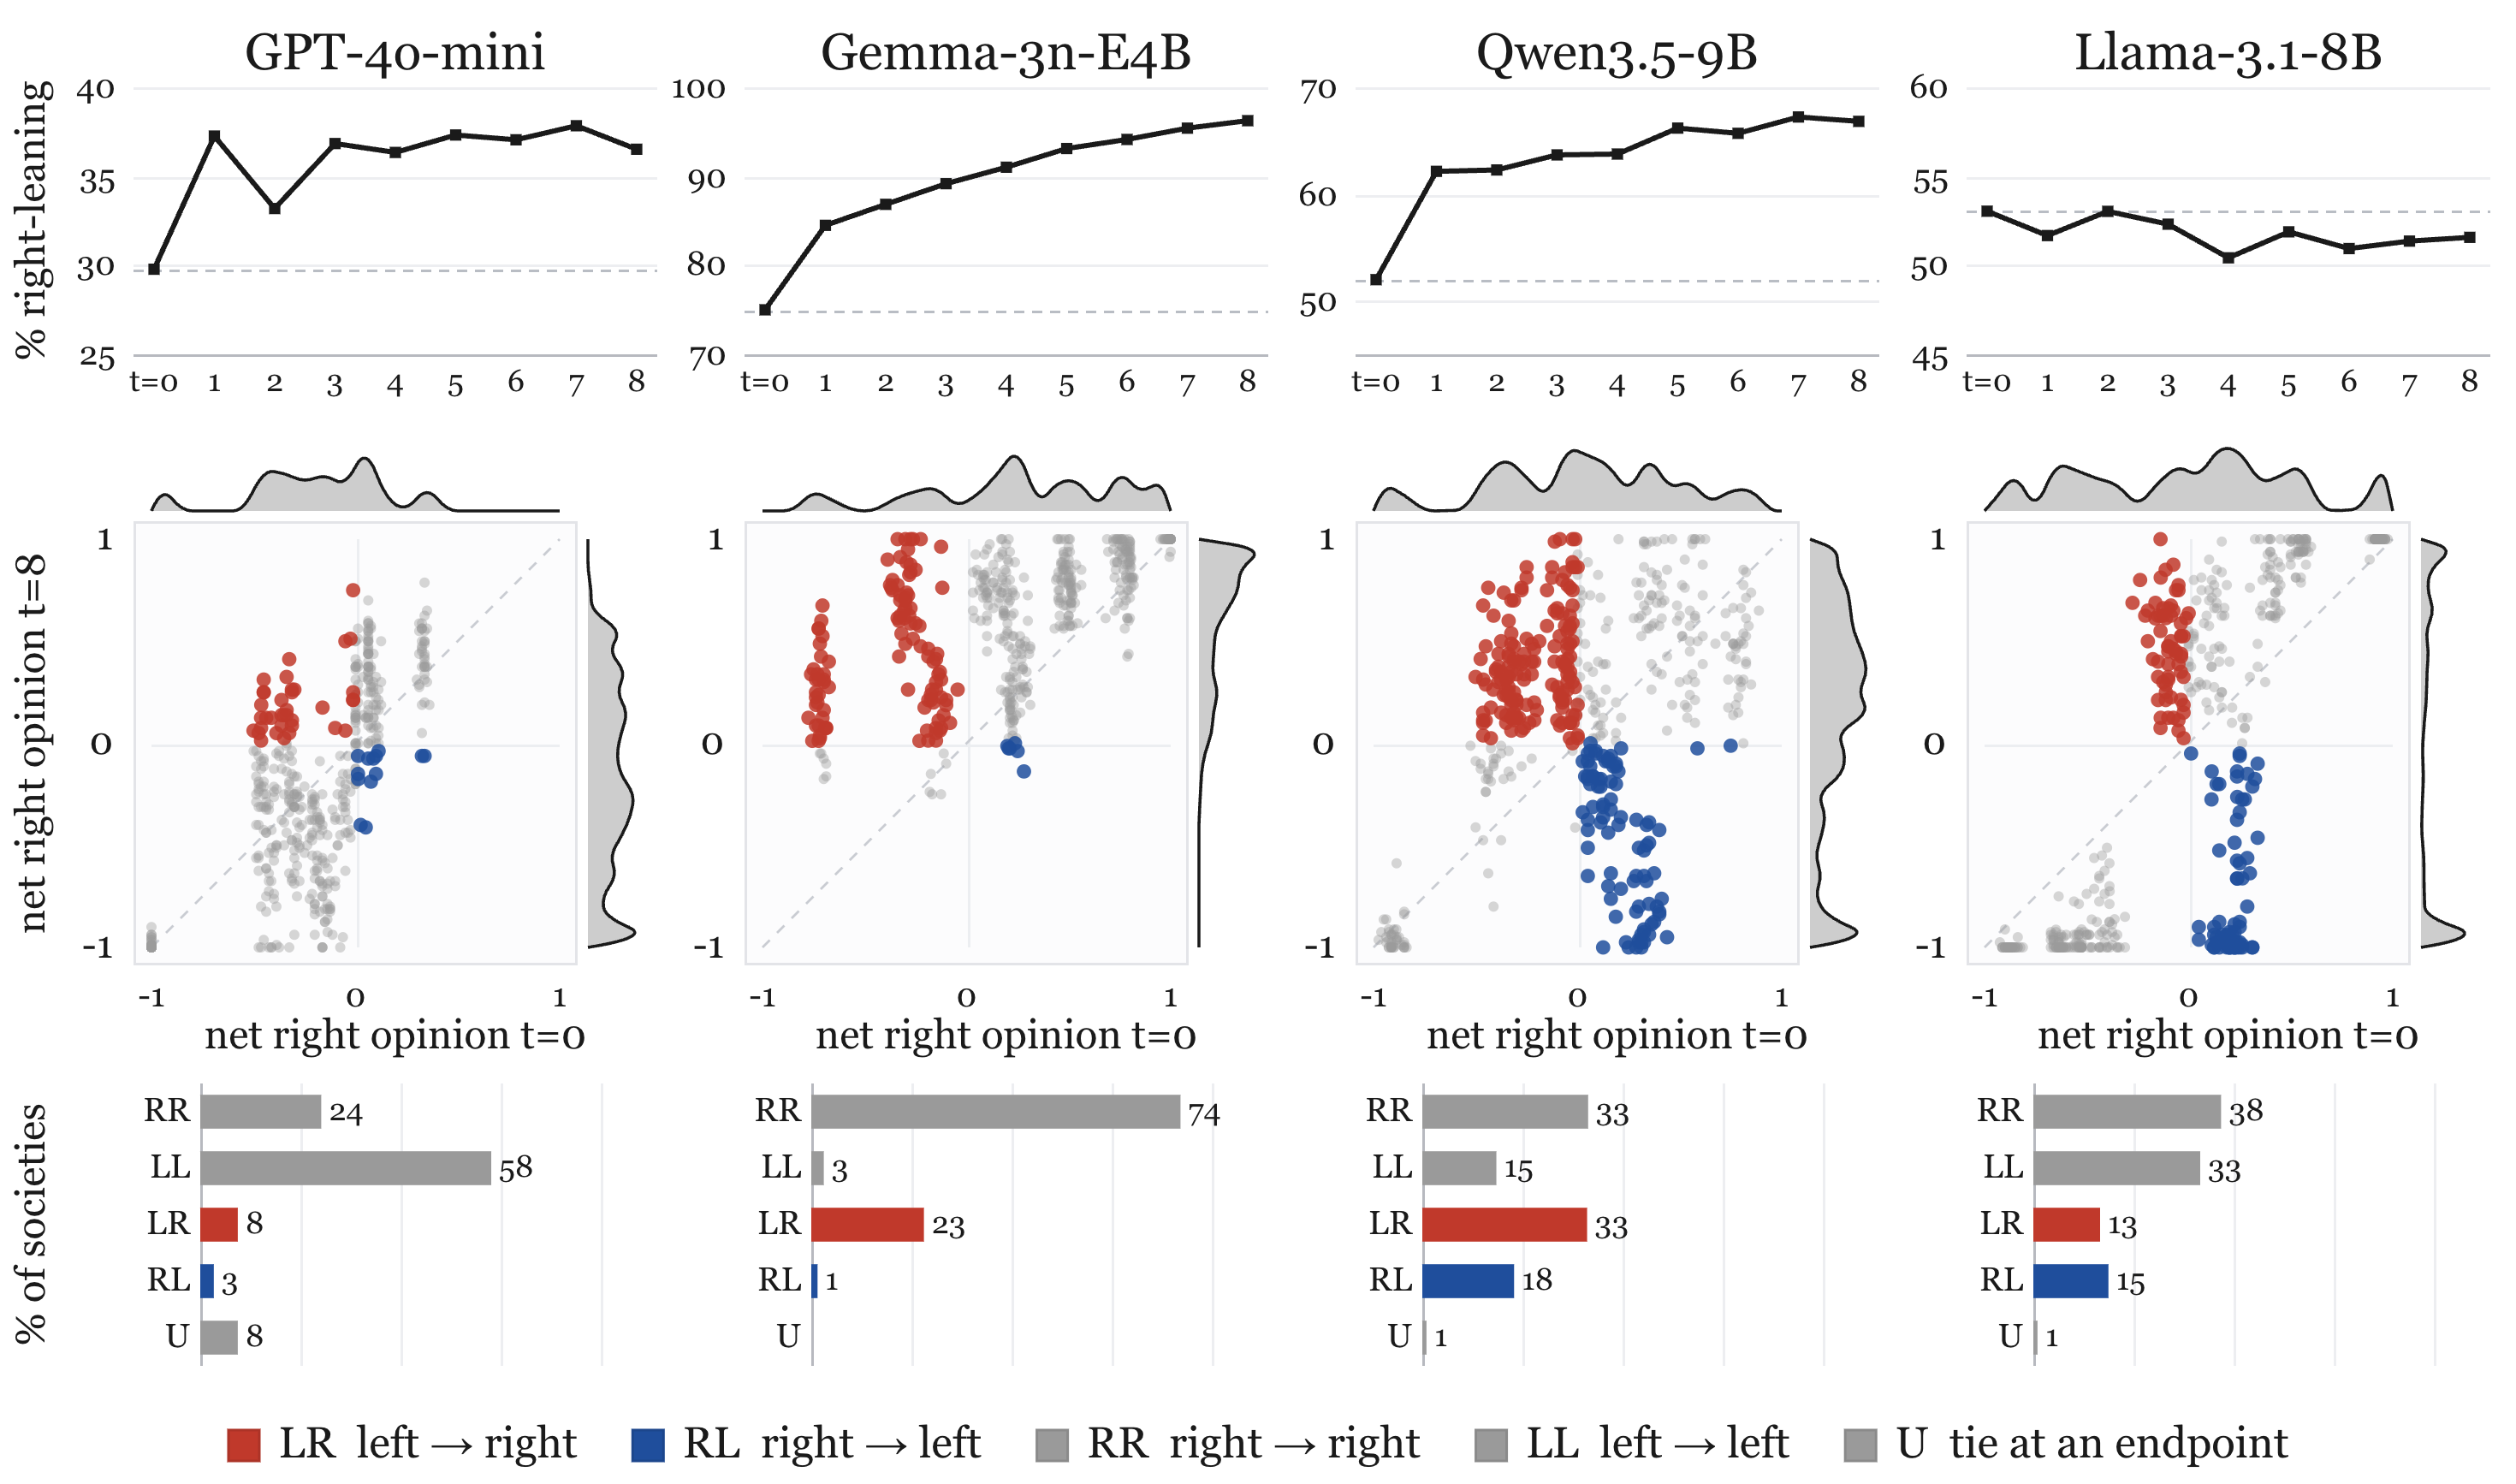
\includegraphics[width=0.99\textwidth]{main/Figures/apx_04_political_lean.png}
        \caption{\textit{Political lean.} How opinions move along the left--right axis on the political statements ($1,920 = 4 \times 12 \times 10 \times 4$ groups from subjective questions only, from signed random graphs and the square and triangular lattices, over both the training- and test-set questions). The statement set is label-balanced (randomly sampling 6 statement with agree leaning left and 6 statement with agree leaning right from Table \ref{tab:political-stance}) so that uniform answer-label bias cancels and does not register as political drift. In a group trajectory, an opinion is represented as right-leaning if net opinion has the same sign as right-leaning opinion. To define which sign a right-leaning opinion has, we labeled the political leaning of agreeing with the statements in our dataset as shown in Table \ref{tab:political-stance}. \emph{Row 1:} $y$-axis: percentage of group trajectories, where the net opinion $n(t)$ has the right-leaning sign at round $t$. $x$-axis: timesteps. \emph{Row 2:} Each point represents a group trajectory, which is plotted based on its initial ($t=0$, $x$-axis) and final ($t=8$, $y$-axis) net opinion $n(t)$ multiplied by the sign of the right-leaning opinion of the questions to get \textit{net right opinion}: $n(t) \cdot y_{r}$, where $y_{r} \in \{-1, +1\}$ denotes the sign of the right-leaning opinion. \emph{Row 3:} Groups switch between being left-leaning and right-leaning at $t=0$ and $t=8$. LL (left$\to$left), LR (left$\to$right), RL (right$\to$left), RR (right$\to$right), and U (undecided, $50\text{-}50$ tie at $t=0$ or $t=8$). The two transition categories LR and RL are highlighted.}
\label{fig:3_Observations_politicallean}
\end{figure}

\subsection{Political Lean of Interacting Agents}\label{apdx:political_lean}



In Section~\ref{sec:truth_seeking}, we explored the truth seeking on objective questions. Here, we present analogous results for subjective questions with a political lean. We labeled the political leaning of each of the political statements in our dataset as shown in Table \ref{tab:political-stance}. In Figure~\ref{fig:3_Observations_politicallean}, we track the fraction of communities whose net opinion sits on the right-leaning side. Three of the four models drift to the right over the eight rounds: Gemma-3n-E4B moves from $75\%$ to $96\%$, Qwen3.5-9B from $52\%$ to $67\%$, and GPT-4o-mini from $30\%$ to $37\%$. Llama-3.1-8B-Instruct is the exception and stays near its starting value of $53\%$, ending marginally lower. The transition counts in the third row make the same point at the level of individual trajectories. Left$\to$right switches outnumber right$\to$left switches by $23\%$ to $1\%$ for Gemma-3n-E4B, $33\%$ to $18\%$ for Qwen3.5-9B, and $8\%$ to $3\%$ for GPT-4o-mini, while Llama-3.1-8B-Instruct is close to symmetric ($13\%$ versus $15\%$). Note that GPT-4o-mini begins strongly left-leaning ($30\%$ right at $t=0$) and still moves rightward under interaction, so the initial distribution of opinions and the direction of drift are separate properties of a community.


\definecolor{leanleft}{HTML}{214E98}   %
\definecolor{leanright}{HTML}{BE3D31}  %

\newcommand{\lleft}{\textcolor{leanleft}{left}}
\newcommand{\lright}{\textcolor{leanright}{right}}
\newcommand{\lnone}{---}

\begin{table}[htbp]
\centering
\small
\setlength{\tabcolsep}{4pt}
\begin{tabularx}{\textwidth}{@{}r l l X l l l@{}}
\toprule
\# & QID & Split & Question & Pole $+$ & Pole $-$ & Agree leans \\
\midrule
1  & \texttt{political\_stance\_0}   & train & Student loan debt should be forgiven by the government     & Agree & Disagree & \lleft  \\
2  & \texttt{political\_stance\_4}   & train & Protest permits infringe on the right to peaceful assembly  & Agree & Disagree & \lnone  \\
3  & \texttt{political\_stance\_11}  & train & Private equity firms harm the companies they acquire        & Agree & Disagree & \lleft  \\
4  & \texttt{political\_stance\_17}  & train & Mandatory vaccination violates bodily autonomy              & Agree & Disagree & \lright \\
5  & \texttt{political\_stance\_62}  & train & Farm subsidies distort markets and should be phased out     & Agree & Disagree & \lright \\
6  & \texttt{political\_stance\_68}  & train & Sanctuary city policies undermine federal immigration law   & Agree & Disagree & \lright \\
7  & \texttt{political\_stance\_72}  & train & Homeschooling should face stricter government oversight     & Agree & Disagree & \lleft  \\
8  & \texttt{political\_stance\_76}  & train & Patent terms should be shortened to encourage innovation    & Agree & Disagree & \lnone  \\
9  & \texttt{political\_stance\_104} & train & Peaceful protest is more effective than civil disobedience  & Agree & Disagree & \lnone  \\
10 & \texttt{political\_stance\_145} & train & Billionaires should not exist in a just society             & Agree & Disagree & \lleft  \\
\addlinespace
11 & \texttt{political\_stance\_156} & test  & Financial transaction taxes would reduce market volatility  & Agree & Disagree & \lleft  \\
12 & \texttt{political\_stance\_231} & test  & Foreign aid spending weakens domestic economic priorities   & Agree & Disagree & \lright \\
13 & \texttt{political\_stance\_232} & test  & The US should maintain military bases around the world      & Agree & Disagree & \lright \\
14 & \texttt{political\_stance\_254} & test  & Stricter gun control laws would reduce violent crime rates  & Agree & Disagree & \lleft  \\
15 & \texttt{political\_stance\_266} & test  & Breaking up big tech companies would increase innovation    & Agree & Disagree & \lnone  \\
16 & \texttt{political\_stance\_353} & test  & Campus speech codes violate First Amendment principles      & Agree & Disagree & \lright \\
17 & \texttt{political\_stance\_361} & test  & NATO expansion provokes conflict and should be halted       & Agree & Disagree & \lnone  \\
18 & \texttt{political\_stance\_363} & test  & Defense spending should be reduced to fund social programs  & Agree & Disagree & \lleft  \\
19 & \texttt{political\_stance\_382} & test  & Critical race theory should be taught in K--12 schools      & Agree & Disagree & \lleft  \\
20 & \texttt{political\_stance\_393} & test  & Nuclear power is essential for achieving clean energy goals & Agree & Disagree & \lnone  \\
\bottomrule
\end{tabularx}
\caption{Political stance items, with train/test split and the direction the ``Agree'' pole leans (\lleft{} / \lright{} / neutral).}
\label{tab:political-stance}
\end{table}
